\usepackage{enumitem}
\usepackage{graphicx}
\usepackage{amsmath}
\usepackage{amssymb}
\usepackage{microtype}
\usepackage{vwcol}  
\usepackage{multicol}
\usepackage{cancel}
\usepackage[top=1cm, left=1.5cm, bottom=0.5cm, right=1.5cm]{geometry}
\usepackage{mathrsfs}
\usepackage{xcolor}
\usepackage{enumitem}
\usepackage{comment}
\usepackage{hyperref}
\usepackage{paracol}
\usepackage{pdfpages}



% Comandos personalizados
\newcommand{\combinat}[2]{\begin{pmatrix} {#1} \\ {#2} \end{pmatrix}}
\newcommand{\magn}[1]{\left[#1 \right]}
\newcommand{\lpn}[1]{\mathscr{L}^{-1}\left\{#1\right\}}
\newcommand{\lp}[1]{\mathscr{L}\left\{#1\right\}}

\newcommand{\frt}[1]{\mathscr{F}\left\{#1\right\}}
\newcommand{\frtn}[1]{\mathscr{F}^{-1}\left\{#1\right\}}

\newcommand{\evalat}[2]{\left. #1 \right|_{{#2}}}
\newcommand{\arccsc}{\operatorname{arccsc}}
\newcommand{\arcsec}{\operatorname{arcsec}}
\newcommand{\arccot}{\operatorname{arccot}}

%    This allows to reference formulas as Section.Subsection. Formula
\newcounter{fmSubSec}[section]
\newcounter{fmCounter}[fmSubSec]
\newcommand{\theformulaCounter}{\arabic{section}.\arabic{fmSubSec}.\arabic{fmCounter}}

\newlist{itemform}{itemize}{1}
\setlist[itemform]{
  label=\textcolor{magenta}{-},
  ref=(\theformulaCounter),
  leftmargin=*,
  noitemsep,
  topsep=0pt,    before=\let\olditem\item\def\item{\stepcounter{fmCounter}\olditem}
}

% Comando para subsecciones (conservando tu nombre)
\newcommand{\fmSubSec}[1]{%
  \stepcounter{fmSubSec}%
  \setcounter{fmCounter}{0}%
  \subsection{#1}%
}

\newenvironment{Figure}
  {\par\medskip\noindent\minipage{\linewidth}}
  {\endminipage\par}
\usepackage{background}

\backgroundsetup{contents=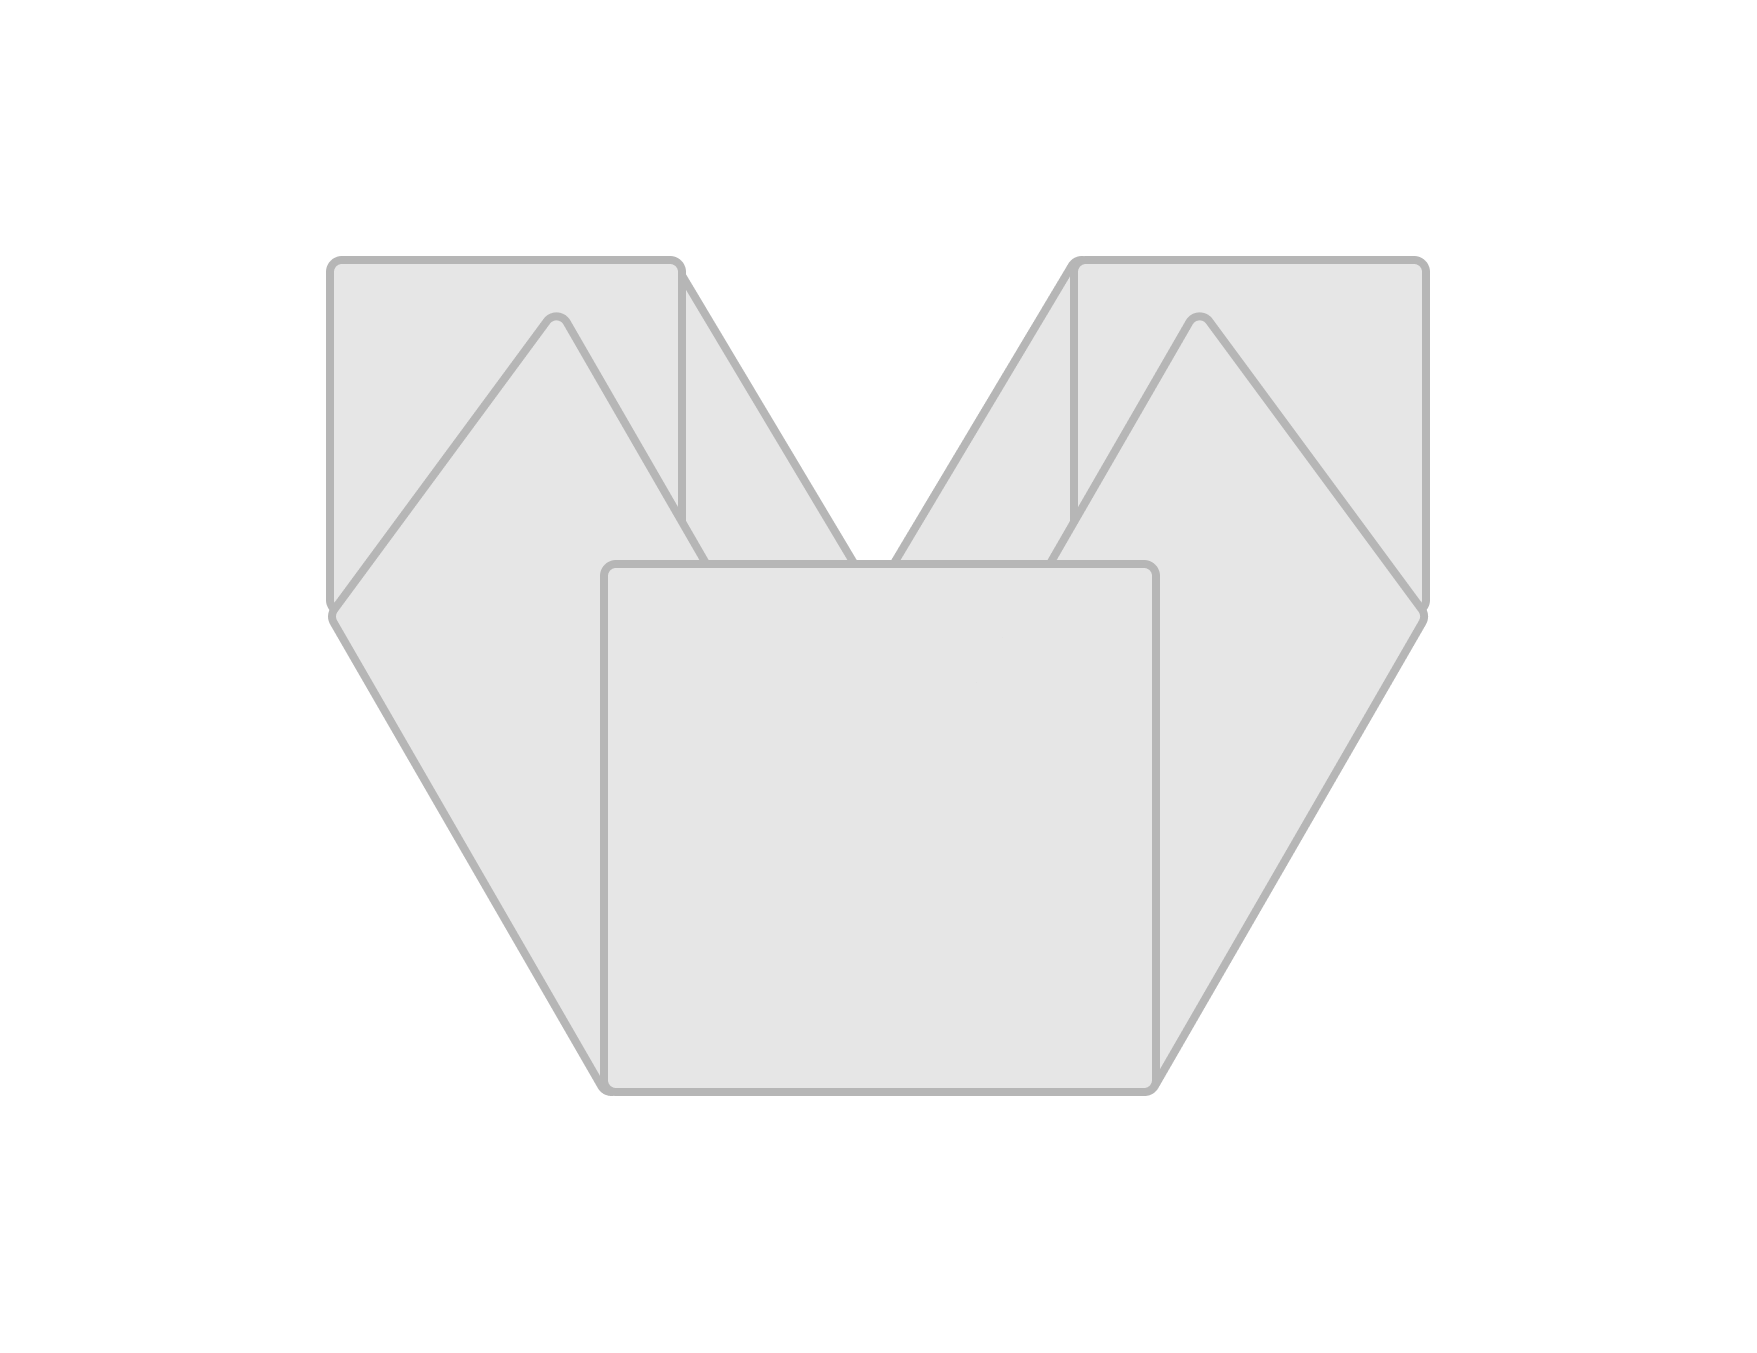
\includegraphics{ALUDAS.png}, scale=1, opacity=0.4,angle =0}

\hypersetup{
    colorlinks=true,
    linkcolor=purple,
    filecolor=magenta,      
    urlcolor=cyan,
    pdftitle={Ultimate Madaf Formulary},
    pdfauthor={Das Reyes},
    bookmarks=true,
    pdfpagemode=FullScreen,
}